\documentclass[11pt, english, fleqn, DIV=15, headinclude, BCOR=2cm]{scrreprt}

\usepackage[
    color,
    bibatend,
]{../../header}

\graphicspath{{./}{../Figures/}}

\newcommand\MZ{M_{\mathrm Z^0}}
\newcommand\electron{\mathrm e^-}
\newcommand\positron{\mathrm e^+}

\usepackage{needspace}

\usepackage{mathtools}
\usepackage{listings}

\lstset{
    basicstyle=\small\ttfamily,
}

\hypersetup{
    pdftitle=
}

\usepackage{longtable}
\usepackage{subcaption}

\usepackage[all]{nowidow}

\subject{Lab report}
\title{Positron lifetime in metals and insulators}
\subtitle{Experiment K225 -- Universität Bonn}
\author{%
    Martin Ueding \\
    \small{\href{mailto:mu@martin-ueding.de}{mu@martin-ueding.de}}
    \and
    Lino Lemmer \\
    \small{\href{mailto:l2@uni-bonn.de}{l2@uni-bonn.de}}
}

\date{\daterange{2016-03-24}{2016-03-25}}

\publishers{Tutor: Martin Urban}

\begin{document}

\maketitle

\begin{abstract}
\end{abstract}

\tableofcontents

\chapter*{Permission to upload}

I, Martin Ueding, would like to scan and upload this lab report with your
corrections to my website \href{http://martin-ueding.de}{martin-ueding.de}.
There, the original lab report as well as the reviewed one will be licensed
under the “\href{http://creativecommons.org/licenses/by-sa/4.0/}{Creative
Commons Attribution-ShareAlike 4.0 International License}”. Is that okay with
you?

Yes $\Box$ \hspace{2cm} No $\Box$

\chapter{Theory}

\section{Metals}

\subsection{Lattice defects}

\subsection{Trapping model}

\subsection{Vacancies}

\section{Positrons}

\subsection{Positron sources}

Our source of positrons will be $\mathrm{^{22}Na}$ throughout the experiment.
Figure~\ref{fig:na22} shows that the sodium decays via a $\betaup^+$-decay or
electron capture into an excited neon isotope. Both decay mechanism are related
via the crossing symmetry and have the same amplitude. Figure~\ref{fig:beta}
shows the first variant. The excited neon will quickly decay into the ground
state and emit a photon. Said photon will mark the creation of the positron.

\begin{figure}
    \centering
    \includegraphics{na22}
    \caption{%
        Decay of $\mathrm{^{22}Na}$.
    }
    \label{fig:na22}
\end{figure}

Due to the creation of the neutrino, the energy spectrum of the positron is
continuous.

\begin{figure}
    \centering
    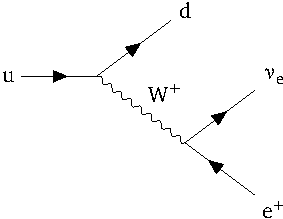
\includegraphics{beta}
    \caption{%
        Feynman diagram for the $\betaup^+$-decay.
    }
    \label{fig:beta}
\end{figure}

\subsection{Positron annihilation}

The tree-level annihilation diagrams are shown in
Figure~\ref{fig:annihilation}. Depending on the relative spin orientations of
the electron and positron, a decay into an even or odd number of photons is
possible. The decay into a single photon is not possible due to
energy-momentum-conservation. Also, the additional creation of two more photon
suppresses the cross section by $\alpha \approx 1/137$. Therefore we can assume
that only decays in two and three photons occur.

\begin{figure}
    \centering
    \begin{subfigure}[c]{0.48\linewidth}
        \centering
        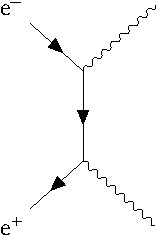
\includegraphics{two-photon}
        \caption{%
            Two photons
        }
        \label{fig:/1}
    \end{subfigure}
    \hfill
    \begin{subfigure}[c]{0.48\linewidth}
        \centering
        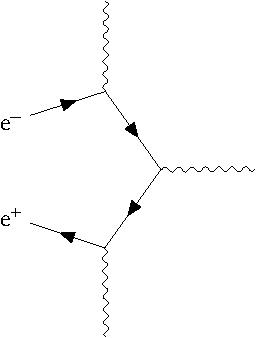
\includegraphics{three-photon}
        \caption{%
            Three photons
        }
        \label{fig:/2}
    \end{subfigure}
    \caption{%
        Decay of a positron into photons.
    }
    \label{fig:annihilation}
\end{figure}

\subsection{Positronium formation}



% TODO Pickof-decay

\section{Measurement technique}

\subsection{LYSO scintillator}

In order to detect the photons, we use a LYSO scintillator. This material is
radioactive itself and provides a built-in energy calibration. The decay scheme
of the radionuclide is shown in Figure~Figure~\ref{fig:scheme-176Lu}

\begin{figure}
    \centering
    \includegraphics{scheme-176Lu}
    \caption{%
        Decay scheme of $^{176}\mathrm{Lu}$ into $^{176}\mathrm{Hf}$.
    }
    \label{fig:scheme-176Lu}
\end{figure}

Photons interact with matter through three channels: Compton scattering at low
charge number $Z$, 

\subsection{Photomultiplier}

\begin{figure}
    \centering
    \includegraphics{photomultiplier}
    \caption{%
        %
    }
    \label{fig:photomultiplier}
\end{figure}

\subsection{Single channel analyzer (SCA)}

\subsection{Time-to-amplitude converter (TAC)}

\subsection{Fast-slow coincidence circuit}

\subsection{Prompt curve}

\chapter{Procedure and Analysis}

\section{Slow circuit setup}

\subsection{LYSO spectrum}

Before adjusting the amplifiers, we have to associate the detected events with
the corresponding transitions. To separate the decay of the ${}^{22}\text{Na}$
from the intrinsic \textsc{lyso} spectrum, we first take the \textsc{lyso}
spectrum of the left and right detectors. In Figure~\ref{fig:lyso} one can
clearly determine the $\SI{596.82}{\kilo\electronvolt}$ cascade decay of the
$6^+$ state of ${}^{176}\text{Hf}$.

\begin{figure}
        \centering
        \begin{subfigure}[c]{.49\linewidth}
                \centering
                \includegraphics{lyso-li}
                \caption{%
                        Left detector.
                }
                \label{fig:lyso-li}
        \end{subfigure}
        \hfill
        \begin{subfigure}[c]{.49\linewidth}
                \centering
                \includegraphics{lyso-re}
                \caption{%
                        Right detector.
                }
                \label{fig:lyso-re}
        \end{subfigure}
        \caption{%
                Intrinsic energy spectrum of the \textsc{lyso} detector.
        }
        \label{fig:lyso}
\end{figure}
        

\subsection{Gain adjust using sodium}

In the sodium spectrum, we expect to see the \SI{511}{\kilo\electronvolt} line
from the annihilation as well as a \SI{1275}{\kilo\electronvolt} line from the
excited neon.

We adjust the gain of the amplifiers such that the sodium spectrum fill the
8192 channels of the \textsc{mca}. The maximum window width of the \textsc{sca}
is not sufficient to let everything through. Also the upper bound for the
\textsc{sca} is below the last channel of the \textsc{mca}. Therefore we cannot
set the amplifier as high as we would like to. For the spectrum, we adjust the
lower bound such that the window covers the two lines we are interested. The
spectra of the left and the right detector are shown in
Figure~\ref{fig:natrium}.

\begin{figure}
        \centering
        \begin{subfigure}[c]{.49\linewidth}
                \centering
                \includegraphics{na-li}
                \caption{%
                        Left detector.
                }
                \label{fig:na-li}
        \end{subfigure}
        \hfill
        \begin{subfigure}[c]{.49\linewidth}
                \centering
                \includegraphics{na-re}
                \caption{%
                        Right detector.
                }
                \label{fig:na-re}
        \end{subfigure}
        \caption{%
                Spectrum of ${}^{22}\text{Na}$. The lines of the detector
                material are also visible.
        }
        \label{fig:natrium}
\end{figure}


We check the coincidence of both \textsc{sca} signals.

\section{Fast circuit setup}

Slow-signal and CFD signal, adjust CFD such that zero-line vanishes.

Look at CFD signals where stop-signal is delayed. We can verify that there is a
\SI{20}{\milli\second} delay between the two.

TAC produces an output.

\section{Time calibration}

SCA coincidence already checked.

TAC+coincidence has very nice overlap.

For a time calibration of our \textsc{mca} we use the coincidence unit as
\textsc{mca}-gate and the \textsc{tac} as input, to take six prompt curves.
Between the measurements another \SI{4}{\nano\second}-delay is interposed. For
the first five prompt curves an acquisition time of about \SI{2}{\minute} is
used.  Together with their fitted Gauss-curves they are shown in
Figure~\ref{fig:prompts_short}. The sixth prompt curve and its fit is shown in
Figure~\ref{fig:prompts_long}. To get a good estimation of the time resolution
the acquisition time is \SI{20}{\minute}.

\begin{figure}
\centering
        \includegraphics{prompts_short}
        \caption{%
                Prompt curves for time calibration. Acquisition time for every
                curve is approximately \SI{2}{\minute}.
        }
        \label{fig:prompts_short}
\end{figure}
        
\begin{figure}
\centering
        \includegraphics{prompts_long}
        \caption{%
                Additional prompt curve for time calibration and time
                resolution estimation. Acquisition time is approximately
                \SI{20}{\minute}.
        }
        \label{fig:prompts_long}
\end{figure}

From the fitted functions we get the mean channel to every delay time. The
results are in Table~\ref{tab:time_gauge_param}. If one plots delay time
against channel number (see Fig.~\ref{fig:time_gauge}) one gets a linear
correlation. Because we don't need absolute time values, just time differences,
only the slope of the fit is of interest for us, which is \SI{<<
time_gauge_slope >>}{\milli\second}.

\begin{table}
        \centering
        \begin{tabular}{SS}
                \toprule
                {delay time/\si{\nano\second}}
                & {mean channel number} \\
                \midrule
                %< for row in time_gauge_param >%
                << ' & '.join(row) >> \\
                %< endfor >%
                \bottomrule
        \end{tabular}
        \caption{%
                Mean channel number of Gauss fit width corresponding delay
                times.
        }
        \label{tab:time_gauge_param}
\end{table}

\begin{figure}
        \centering
        \includegraphics{time_gauge}
        \caption{%
                Time calibration of \textsc{mca}-channels. The error bars for
                the channel number are so small, they hide behind the
                markers.
        }
        \label{fig:time_gauge}
\end{figure}
        

The last prompt curve has a standard deviation of \num{<< width_6 >>}. From
this we get $\textsc{fwhm} = \num{<< FWHM_6 >>}$. With the slope of the time
calibration fit we get a resolution of \SI{<< time_resolution >>}{\nano\second}.

\section{Adjusting SCA windows}

Selecting \SI{1275}{\kilo\electronvolt} line on start-side.

Checking SCA coindicence, has nice overlap.

Check TAC+coincidence, has nice overlap.

\section{Indium sample}

\subsection{Vacancy formation enthalpy}

\section{Acrylic glass sample}

\end{document}

% vim: spell spelllang=en_us tw=79
